\section{Chisel} \label{app:chisel}


%%%%%%%%%%%%%%%%%%%%%%%
\subsection{Introduction}
%%%%%%%%%%%%%%%%%%%%%%%
Chisel (\textbf{C}onstructing \textbf{H}ardware \textbf{I}n a \textbf{S}cala \textbf{E}mbedded \textbf{L}anguage) is a hardware design language embedded within Scala. It allows hardware designers to write complex, parameterizable, and reusable hardware components using high-level programming constructs \cite{bachrach2012chisel}. 

This Appendix is a very brief introduction to Chisel primarily for designers to reference features quickly. For processor design, \citep{chisel:book} is a highly recommended free book. The Chisel Cheat Sheet is also helpful \cite{chiselcheatsheet}.

%%%%%%%%%%%%%%%%%%%%%%%%%%%%
\subsection{Key Features of Chisel}
%%%%%%%%%%%%%%%%%%%%%%%%%%%%
Chisel is a domain-specific language (DSL) for hardware design, using Scala's object-oriented and functional programming features \cite{chisel-doc}. It compiles to synthesizable Verilog, integrating with traditional hardware development flows.

\paragraph{Hardware Construction Language.} High-level abstractions for hardware components.
\paragraph{Parameterization.} Easy creation of generic and reusable modules.
\paragraph{Strong Typing.} Reduces errors through rigorous type checking.
\paragraph{Functional Programming.} Utilizes Scala's functional paradigms for concise code.


%%%%%%%%%%%%%%%%%
\subsection{Syntax}
%%%%%%%%%%%%%%%%

%************************
\subsection{Scala Basics}
%************************
Understanding basic Scala syntax is needed for Chisel programming \cite{odersky2008programming}.

\paragraph{Immutable Variables (\texttt{val}).} Cannot be reassigned.
\paragraph{Mutable Variables (\texttt{var}).} Can be reassigned.
\paragraph{Functions (\texttt{def}).} Defined using the \texttt{def} keyword.
\paragraph{Classes and Objects.} Used to define hardware modules and singletons.

%******************************
\subsection{Import Statements}
%*****************************
Include necessary Chisel libraries at the beginning of your file:

\begin{chiselcode}
import chisel3._
import chisel3.util._    
\end{chiselcode}

%%%%%%%%%%%%%%%%%%%%
\subsection{Data Types}
%%%%%%%%%%%%%%%%%%%%
Chisel provides specialized data types for hardware representation \cite{chisel-doc}.

%***********************
\subsection{Base Types}
%**********************
\paragraph{Bool.} Single-bit boolean (\texttt{true}/\texttt{false}). Declaration: \texttt{val myBool = Bool()}

\paragraph{UInt.} Unsigned integer with specified width. Declaration: \texttt{val myUInt = UInt(8.W)}

\paragraph{SInt.} Signed integer with specified width. Declaration: \texttt{val mySInt = SInt(16.W)}

\paragraph{FixedPoint.} Fixed-point number with total and fractional bits. Declaration: \texttt{val myFixed = FixedPoint(16.W, 8.BP)}

\paragraph{Clock.} Represents a clock signal.

\paragraph{Reset.} Represents a reset signal.

%****************************
\subsection{Aggregate Types}
%***************************
\paragraph{Bundle.} Custom data structures combining multiple fields. Declaration: \texttt{class MyBundle extends Bundle \{ val a = UInt(8.W) \}}

\paragraph{Vec.} Indexable collection of elements of the same type. Declaration: \texttt{val myVec = Vec(4, UInt(8.W))}

%********************
\subsection{Literals} 
%********************
\paragraph{Unsigned Integer.}  \texttt{10.U}, \texttt{3.U(8.W)}

\paragraph{Signed Integer.} \texttt{-5.S}, \texttt{-2.S(8.W)}

\paragraph{Boolean.} \texttt{true.B}, \texttt{false.B}

%*********************
\subsection{Operators} 
%*********************
\paragraph{Arithmetic (\texttt{+, -, *, /, \%}).} \texttt{+} (addition), \texttt{-} (subtraction), \texttt{*} (multiplication), \texttt{/} (division), \texttt{\%} (modulo operation)

\paragraph{Logical (\texttt{\&, |, \^, !}).} \texttt{\&} (logical AND), \texttt{|} (logical OR), \texttt{\^{}} (logical XOR), \texttt{!} (logical NOT)

\paragraph{Comparison (\texttt{===, =/=, <, <=, >, >=}).} \texttt{===} (equal to), \texttt{=/=} (not equal to), \texttt{<} (less than), \texttt{<=} (less than or equal to), \texttt{>} (greater than), \texttt{>=} (greater than or equal to)

\paragraph{Bitwise Reduction (\texttt{\&, |, \^}).} \texttt{\&} (bitwise AND reduction), \texttt{|} (bitwise OR reduction), \texttt{\^{}} (bitwise XOR reduction). These operators are applied to a single operand.

\paragraph{Shift (\texttt{<<, >>}).} \texttt{<<} (left shift), \texttt{>>} (right shift)

%%%%%%%%%%%%%%%%%%%%%%%%%%%%%%%
\subsection{Modules and Hierarchy}
%%%%%%%%%%%%%%%%%%%%%%%%%%%%%%%
%****************************
\subsection{Defining Modules}
%****************************
Modules are defined by extending the \texttt{Module} class \cite{chisel-doc}.

\begin{chiselcode}
class MyModule extends Module {
  // Module implementation
}    
\end{chiselcode}

%******************************
\subsection{Input/Output Ports}
%*******************************
Ports are declared using the \texttt{IO} method with a \texttt{Bundle}.
\begin{chiselcode}
class MyModule extends Module {
  val io = IO(new Bundle {
    val in  = Input(UInt(8.W))
    val out = Output(UInt(8.W))
  })
  // Module logic
}    
\end{chiselcode}

%*********************************
\subsection{Instantiating Modules}
%*********************************
Modules can be instantiated within other modules.
\begin{chiselcode}
val subModule = Module(new SubModule)
subModule.io.in := io.in
io.out := subModule.io.out
\end{chiselcode}

%*********************************
\subsection{Parameterized Modules}
%*********************************
Modules can be parameterized for reusability.
\begin{chiselcode}
class MyModule(val width: Int) extends Module {
  val io = IO(new Bundle {
    val in  = Input(UInt(width.W))
    val out = Output(UInt(width.W))
  })
  // Module logic
}    
\end{chiselcode}

%%%%%%%%%%%%%%%%%%%%%%%%%%%%%%
\subsection{Wires and Registers}
%%%%%%%%%%%%%%%%%%%%%%%%%%%%%
Wires represent combinational logic signals \cite{chisel-doc}.
\begin{chiselcode}
val tempWire = Wire(UInt(8.W))
tempWire := io.in + 1.U    
\end{chiselcode}

Registers store state across clock cycles.
\begin{itemize}
    \item \texttt{Reg}: Creates a register without an initial value.
        \newline Declaration: \texttt{val myReg = Reg(UInt(8.W))}
    \item \texttt{RegInit}: Creates a register with an initial value.
        \newline Declaration: \texttt{val myReg = RegInit(0.U(8.W))}
\end{itemize}

Registers are updated using non-blocking assignment.
\begin{chiselcode}
myReg := myReg + 1.U    
\end{chiselcode}

%%%%%%%%%%%%%%%%%%%%%%%%%%%%%
\subsection{Control Structures}
%%%%%%%%%%%%%%%%%%%%%%%%%%%%%

%************************************
\subsection{\texttt{when} Statements}
%************************************
Conditional hardware execution.
\begin{chiselcode}
when (condition) {
  // Actions when condition is true
} .elsewhen (anotherCondition) {
  // Actions when anotherCondition is true
} .otherwise {
  // Actions when all conditions are false
}
\end{chiselcode}

%**************************************
\subsection{\texttt{switch} Statements}
%**************************************
Multi-way conditional execution.
\begin{chiselcode}
switch(selector) {
  is(value1) {
    // Actions for value1
  }
  is(value2) {
    // Actions for value2
  }
}
\end{chiselcode}

%*********************************
\subsection{\texttt{Mux} Function}
%*********************************
Multiplexer for conditional selection.
\begin{chiselcode}
val result = Mux(condition, trueValue, falseValue)
\end{chiselcode}

%*******************
\subsection{Loops}
%******************
Used for hardware generation, not for creating sequential logic \cite{chisel-tutorial}.
\begin{chiselcode}
for (i <- 0 until n) {
  // Generate n instances of hardware
}
\end{chiselcode}

%%%%%%%%%%%%%%%%%%%%%%%%%%%%%%%%%%%
\subsection{Functions and Procedures}
%%%%%%%%%%%%%%%%%%%%%%%%%%%%%%%%%%%
%******************************
\subsection{Defining Functions}
%******************************
Functions encapsulate reusable logic.
\begin{chiselcode}
def add(a: UInt, b: UInt): UInt = {
  a + b
}
\end{chiselcode}

%*******************************
\subsection{Invoking Functions}
%******************************
\begin{chiselcode}
val sum = add(io.in1, io.in2)
\end{chiselcode}

%%%%%%%%%%%%%%%%%%%%%%%%%%%%%
\subsection{Parameterized Types}
%%%%%%%%%%%%%%%%%%%%%%%%%%%%%%
Types can be parameterized for flexibility.
\begin{chiselcode}
def myFunction[T <: Data](in: T): T = {
  // Function body
}
\end{chiselcode}

The function \texttt{myFunction} is a generic method in Chisel that operates on a parameterized data type \texttt{T}. The parameter \texttt{T} is constrained to extend the \texttt{Data} type, which is the base class for all hardware types in Chisel, such as \texttt{UInt}, \texttt{SInt}, or \texttt{Bundle}. This ensures that \texttt{myFunction} can accept any valid Chisel hardware type as its input. The method takes a single input argument \texttt{in} of type \texttt{T} and returns a value of the same type \texttt{T}. While the function body is not specified, this structure is commonly used to define reusable, type-safe operations on hardware constructs, enabling modular and flexible hardware design.

%%%%%%%%%%%%%%%%%%%%%%%%%%
\subsection{Generic Modules}
%%%%%%%%%%%%%%%%%%%%%%%%%%
Modules can be generic over data types.
\begin{chiselcode}
class MyGenericModule[T <: Data](genType: T) extends Module {
  val io = IO(new Bundle {
    val in  = Input(genType)
    val out = Output(genType)
  })
  // Module logic
}
\end{chiselcode}

The \texttt{MyGenericModule} class is a parameterized hardware module in Chisel. It extends the \texttt{Module} base class and takes a type parameter \texttt{T}, constrained to be a subtype of \texttt{Data}, which ensures that it can represent any Chisel hardware type such as \texttt{UInt}, \texttt{SInt}, or custom \texttt{Bundle}s. The parameter \texttt{genType} is passed to the constructor and defines the specific type of data the module will operate on. Inside the module, the \texttt{io} interface is declared using a \texttt{Bundle}, containing an input port \texttt{in} and an output port \texttt{out}, both of which use the generic type \texttt{genType}. This design allows the module to be highly reusable and adaptable, as it can handle different data types depending on the parameter provided during instantiation. The comment \texttt{// Module logic} indicates where the functional implementation of the module would be added.


%%%%%%%%%%%%%%%%%%%%%%%%%%%%%%%%%%%%%%%%%%
\subsection{Hardware Construction in Chisel}
%%%%%%%%%%%%%%%%%%%%%%%%%%%%%%%%%%%%%%%%%

%***********************************
\subsection{Vectors (\texttt{Vec})}
%***********************************
Indexable collections of elements.
\begin{chiselcode}
val myVec = VecInit(Seq.fill(4)(0.U(8.W)))
myVec(0) := io.in
\end{chiselcode}

%************************************
\subsection{Memories (\texttt{Mem})}
%***********************************
Memory elements for storage.
\begin{chiselcode}
val myMem = Mem(1024, UInt(8.W))
val dataOut = myMem.read(addr)
myMem.write(addr, dataIn)
\end{chiselcode}

%*******************
\subsection{Bundles}
%*******************
Custom data structures grouping multiple fields.
\begin{chiselcode}
class MyBundle extends Bundle {
  val field1 = UInt(8.W)
  val field2 = Bool()
}
\end{chiselcode}

%%%%%%%%%%%%%%%%%%%%%%%%%%%%%%%%%%%
\subsection{Testing and Verification}
%%%%%%%%%%%%%%%%%%%%%%%%%%%%%%%%%%
\subsection{ChiselTest Framework}
%********************************
ChiselTest provides tools for testing Chisel modules \cite{chiseltest}.
\begin{chiselcode}
import chiseltest._
import org.scalatest.flatspec.AnyFlatSpec

class MyModuleTest extends AnyFlatSpec with ChiselScalatestTester {
  "MyModule" should "perform correctly" in {
    test(new MyModule) { c =>
      c.io.in.poke(0.U)
      c.clock.step(1)
      c.io.out.expect(0.U)
    }
  }
}
\end{chiselcode}

%**********************
\subsection{Assertions}
%**********************
In-module checks using \texttt{assert}.
\begin{chiselcode}
assert(io.out === expectedValue)
\end{chiselcode}

%%%%%%%%%%%%%%%%%%%%%%%%%%%%%%%%%
\subsection{Peculiarities of Chisel}
%%%%%%%%%%%%%%%%%%%%%%%%%%%%%%%%%%
%**************************************
\subsection{Chisel is Embedded in Scala}
%**************************************
Chisel code is Scala code. This means:

\begin{itemize}
    \item Full access to Scala's features.
    \item Potential confusion between hardware constructs and software constructs.
\end{itemize}

%***********************************
\subsection{Delayed Execution Model}
%***********************************
Chisel builds a hardware graph during elaboration, which may lead to unexpected behavior if side effects are not managed properly \cite{chisel-doc}.

%********************************
\subsection{Assignment Operators}
%********************************
\begin{itemize}
    \item \texttt{:=} Used for updating hardware signals.
    \item \texttt{=} Used for variable assignment in Scala.
\end{itemize}

%***********************
\subsection{Type System}
%***********************
Chisel enforces strict type checking, which may differ from SystemVerilog or VHDL.

%******************************************************
\subsection{Combining Hardware and Software Constructs}
%******************************************************
Be cautious when mixing Scala control structures (e.g., \texttt{if}, \texttt{for}) with Chisel constructs (\texttt{when}, \texttt{switch}) \cite{chisel-tutorial}.

%*****************************************
\subsection{Hardware vs. Software Mindset}
%*****************************************
Designers must think in terms of hardware concurrency, even when writing code that resembles sequential software.

%%%%%%%%%%%%%%%%%%%%%%%%%%%%%%%%%%%%%%
\subsection{Installing Chisel on Ubuntu}
%%%%%%%%%%%%%%%%%%%%%%%%%%%%%%%%%%%%%%%

%*******************************************
\subsection{Scripts Directory}
%******************************************
If you are running Ubuntu, {\tt RTL/Scripts} contains useful installation scripts that automate the installation process.


%******************************************
\subsection{Install a Java Development Kit}
%*******************************************
Chisel is built on Scala, which requires the Java Development Kit (JDK). You have two options to install and manage the JDK.

%**************************************
\subsubsection{Install the Default JDK}
%**************************************        
\begin{bashcode}
sudo apt update && sudo apt install default-jdk
\end{bashcode}

%*********************
\subsubsection{SDKMan}
%*********************

SDKMAN! is a tool for managing parallel versions of Software Development Kits (SDKs) such as Java, Groovy, Kotlin, and more. It simplifies the installation, update, and switching between SDK versions.

\paragraph*{Installation}

To install SDKMAN!, open a terminal and run the following command:
\begin{bashcode}
     curl -s "https://get.sdkman.io" | bash       
\end{bashcode}

Add the following line to your .bashrc configuration file:
\begin{bashcode}
export SDKMAN_DIR="$HOME/.sdkman"
source "$SDKMAN_DIR/bin/sdkman-init.sh"
source ~/.bashrc
\end{bashcode}

After installation, restart your terminal or run:
\begin{bashcode}
    source "\$HOME/.sdkman/bin/sdkman-init.sh"        
\end{bashcode}

Verify the installation by running:
\begin{bashcode}
 sdk version    
\end{bashcode}       

\paragraph*{Using SDKMAN!}
Here are some common commands:

List All Available Java Versions:
\begin{bashcode}    
sdk list java
\end{bashcode}

Install a Specific Version
\begin{bashcode}
sdk install java 23-oracle   
\end{bashcode}

Set a Default Version
\begin{bashcode}
sdk default java 23-oracle    
\end{bashcode}

Switch Java Versions:
\begin{bashcode}
sdk use java 23-oracle    
\end{bashcode}

%******************************************
\subsection{Install Scala Build Tool (sbt)}
%******************************************
\begin{bashcode}
echo "deb https://repo.scala-sbt.org/scalasbt/debian all main" | \
sudo tee /etc/apt/sources.list.d/sbt.list && \
curl -sL "https://keyserver.ubuntu.com/pks/lookup? \ 
op=get&search=0x99E82A75642AC823" | \
sudo apt-key add && \
sudo apt update && \
sudo apt install sbt
\end{bashcode}


\paragraph{Clone this book}
Or use the template at 
\begin{bashcode}
https://github.com/chipsalliance/chisel
\end{bashcode}

\paragraph{Build and Run Your Chisel Project}
Navigate to your project's directory and use sbt to compile and run it:
\begin{bashcode}
cd your-chisel-project && sbt test
\end{bashcode}

%******************************
\subsection{Install Verilator}
%******************************
\begin{bashcode}
sudo apt-get install verilator
\end{bashcode}

For any operating system other than Ubuntu, see: https://verilator.org/guide/latest/install.html.

%******************************
\subsection{Install gtkwave}
%******************************
To view the waveforms created by verilator, instal gtkwave.
\begin{bashcode}
sudo apt-get install gtkwave
\end{bashcode}

%******************************
% \subsection{Install Vivado}
%******************************


%******************************
% \subsection{Install OpenLane}
%******************************

%******************************
% \subsection{Install OSS CAD Suite}
%******************************

%******************************
% \subsection{Install circt (firtool)}
%******************************

%%%%%%%%%%%%%%%%%%%%%%%%%%%%%
\subsection{Example Walkthrough}
%%%%%%%%%%%%%%%%%%%%%%%%%%%%%
Assuming you have cloned this book (Structured Computer Architecture), you will find the Chisel source files in the RTL/Chisel directory at the top level of the repository.

%***************************
\subsection{Key Directories}
%***************************
\begin{verbatim}
    RTL/Scripts:                              Installation scripts for Ubuntu 24.04
    RTL/Chisel/src/main/scala/scabook:        Chisel source files
    RTL/Chisel/test/scala/scabook:            Chisel test harness files
    RTL/Chisel/generated_verilog_clean:       SystemVerilog generated by Chisel 
    RTL/Chisel/generated_verlilog_annotated:  SystemVerilog with debug symbols
    RTL/Chisel/verilog_testbench:             Verilator C++ testbench files
\end{verbatim}

%***************************
\subsection{Run Chisel Test}
%***************************
The following very simple design generates a waveform
\includechiselcode[caption={Waveform Generator Code (Chisel)}, label={lst:chisel_waveformgenerator2}]{\chiselSourceDir/waveFormGenerator.scala}

The testbench for the code is:
\includechiselcode[caption={Waveform Generator Testbench Code (Chisel)}, label={lst:chisel_waveformgeneratortestbench}]{\chiselTestBenchSourceDir/waveFormGeneratorSpec.scala}

%*****************************
\subsection{Run the Testbench}
%*****************************
If you have cloned the textbook, build.sbt will be in your Chisel/ directory.
\includechiselcode[caption={Waveform Generator Testbench Code (Chisel)}, label={lst:build_sbt}]{RTL/Chisel/build.sbt}

The following commands will run the test bench
\begin{bashcode}
cd RTL/Chisel/
sbt test
\end{bashcode}

The IDE being used is Visual Studio Code with the Scala(Metals) extension installed. Your output should look something like:
\begin{bashcode}
(base) jglossner@jglossner-Alienware-Aurora-R7:~/GitRepos/Structured_Computer_Architecture/Chisel\$ sbt test
downloading sbt launcher 1.10.6
[info] welcome to sbt 1.10.5 (Oracle Corporation Java 23)
[info] loading settings for project chisel-build-build from metals.sbt ...
[info] loading project definition from /home/jglossner/GitRepos/Structured_Computer_Architecture/Chisel/project/project
[info] loading settings for project chisel-build from metals.sbt ...
[info] loading project definition from /home/jglossner/GitRepos/Structured_Computer_Architecture/Chisel/project
[success] Generated .bloop/chisel-build.json
[success] Total time: 1 s, completed Nov 30, 2024, 11:12:37 AM
[info] loading settings for project root from build.sbt ...
[info] set current project to %NAME% (in build file:/home/jglossner/GitRepos/Structured_Computer_Architecture/Chisel/)
[info] WaveFormGeneratorSpec:
[info] - WaveFormGenerator should generate the correct waveforms
[info] GCDSpec:
[info] - Gcd should calculate proper greatest common denominator
[info] Run completed in 8 seconds, 403 milliseconds.
[info] Total number of tests run: 2
[info] Suites: completed 2, aborted 0
[info] Tests: succeeded 2, failed 0, canceled 0, ignored 0, pending 0
[info] All tests passed.
[success] Total time: 9 s, completed Nov 30, 2024, 11:12:46 AM
\end{bashcode}

%*****************************************
\subsection{Generate Clean System Verilog}
%*****************************************
The only difference between the clean SystemVerilog and the annotated version is the commented out code.

For clean SystemVerilog:
\begin{chiselcode}
object WaveFormGenerator extends App {
  ChiselStage.emitSystemVerilogFile(
    new WaveFormGenerator,
    //Array("--target-dir", "generated")
    firtoolOpts = Array("-disable-all-randomization", "-strip-debug-info"),
  )
}
\end{chiselcode}

Run the SystemVerilog generator from the Chisel/ directory
\begin{bashcode}
sbt run
\end{bashcode}

This will produce
\includeverilogcode[caption={Clean SystemVerilog Code Produced by Chisel}, label={lst:chisel_waveformgeneratorcleanverilog}]{\verilogGeneratedByChiselSourceDir/WaveFormGenerator.v}

%***************************************************
\subsection{Generate Annotated/Debug System Verilog}
%***************************************************
This code will put the SystemVerilog simulation code directly into a generated folder
\begin{chiselcode}
object WaveFormGenerator extends App {
  ChiselStage.emitSystemVerilogFile(
    new WaveFormGenerator,
    Array("--target-dir", "generated")
    //firtoolOpts = Array("-disable-all-randomization", "-strip-debug-info"),
  )
}
\end{chiselcode}

The annotated/debug SystemVerilog generated code should look like:
\includeverilogcode[caption={Annotated SystemVerilog Code Produced by Chisel}, label={lst:chisel_waveformgeneratorannotatedverilog}]{RTL/Chisel/generators/generated/systemverilog_annotated/WaveFormGenerator.v}

%***********************************************
\subsection{Verilator C++ Test Driver} \label{sub:verilator_test_driver}
%***********************************************
Create a Verilator C++ test driver. It is in Chisel/verilator\_testbench
\includecppcode[caption={Verilator Testbench for WaveFormGenerator}, label={lst:verilator_waveformgenerator_testbench}]{\verilatorSourceDir/WaveFormGenerator_testbench.cpp}

From the Chisel/verilator\_testbench, execute:
\begin{bashcode}
verilator --cc ../generated_verilog_annotated/WaveFormGenerator.sv --exe WaveFormGenerator_testbench.cpp --trace
make -C obj_dir -f VWaveFormGenerator.mk VWaveFormGenerator   
\end{bashcode}

This will output the executable in Chisel/verilator\_testbench/obj\_dir

Execute the WaveFormGenerator program create in the obj\_dir
\begin{bashcode}
obj_dir/VWaveFormGenerator
\end{bashcode}

This will create a vcd file that can be displayed with gtkwave
\begin{bashcode}
gtkwave waveform.vcd    
\end{bashcode}

\begin{figure}[H]
    \centering
    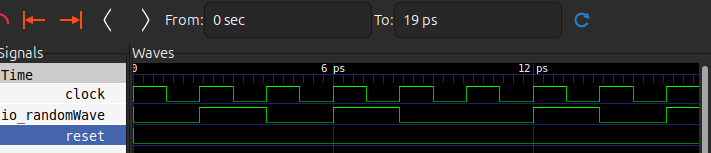
\includegraphics[width=\textwidth]{Images/verilator_waveformgenerator_screenshot.png} 
    \caption{Waveforms generated for a Verilator SystemVerilog simulation}
    \label{fig:verilator_wave2}
\end{figure}

%%%%%%%%%%%%%%%%%%%%%%%%%%%0
\subsection{Vivado Execution}
%%%%%%%%%%%%%%%%%%%%%%%%%%%%
Vivado is a comprehensive FPGA design suite developed by Xilinx. It integrates various tools for hardware design, simulation, synthesis, implementation, and debugging. Vivado supports Verilog, SystemVerilog, and VHDL for both design and simulation.

%**********************************
\subsection{Steps to Use Vivado}
%**********************************
\begin{enumerate}
    \item \textbf{Create a Project:}
    \begin{itemize}
        \item Open Vivado and create a new project.
        \item Specify the project type (RTL or post-synthesis).
        \item Add source files (e.g., Verilog, SystemVerilog, or VHDL).
    \end{itemize}

    \item \textbf{Write or Import a Testbench:}
    \begin{itemize}
        \item Add a testbench to simulate your design.
        \item Set the testbench as the top module for simulation.
    \end{itemize}

    \item \textbf{Simulate the Design:}
    \begin{itemize}
        \item Use the Vivado simulator to run behavioral simulations.
        \item Analyze the results in the waveform viewer.
    \end{itemize}

    \item \textbf{Synthesize and Implement:}
    \begin{itemize}
        \item Perform synthesis to generate a netlist.
        \item Run implementation to map the design to the FPGA.
    \end{itemize}

    \item \textbf{Generate a Bitstream:}
    \begin{itemize}
        \item Create a bitstream file to program the FPGA.
    \end{itemize}
\end{enumerate}

%************************************
\subsection{Key Features of Vivado}
%************************************
\begin{itemize}
    \item Supports advanced FPGA features such as high-speed transceivers and DSP blocks.
    \item Built-in waveform viewer for debugging simulations.
    \item Comprehensive support for Xilinx devices.
\end{itemize}

%********************************************
\subsection{Comparison of Vivado and Verilator}
%********************************************
Vivado and Verilator are both widely used in hardware design, but they cater to different needs. Below is a detailed comparison:

\begin{table}[htbp]
\renewcommand{\arraystretch}{2} % Adjust the row height (1.5x default)
\centering
\begin{tabular}{@{}p{4cm}p{6cm}p{6cm}@{}}
\toprule
\textbf{Feature}              & \textbf{Vivado}                                & \textbf{Verilator}                              \\ \midrule
\textbf{Purpose}              & Comprehensive FPGA design suite                & High-speed cycle-accurate simulation tool       \\
\textbf{Languages Supported}  & Verilog, SystemVerilog, VHDL                   & Verilog, SystemVerilog                         \\
\textbf{Test Driver Language} & HDL (Verilog/SystemVerilog/VHDL)               & C++ (or SystemC for advanced simulations)      \\
\textbf{Simulation Speed}     & Moderate (event-driven simulator)              & Very high (compiled C++ simulation)            \\
\textbf{Waveform Viewer}      & Built-in (integrated with simulation)          & Requires external tools like GTKWave (VCD)     \\
\textbf{FPGA Synthesis}       & Yes                                           & No                                             \\
\textbf{FPGA Targeting}       & Xilinx FPGAs                                   & Not applicable                                 \\
\textbf{Debugging Features}   & Integrated debugging and timing analysis tools & Debugging through C++ or external tools        \\
\textbf{Open Source}          & No (proprietary software)                      & Yes (GPL-licensed)                             \\ \bottomrule
\end{tabular}
\caption{Comparison of Vivado and Verilator}
\label{tab:vivado_vs_verilator}
\end{table}

\subsection*{When to Use Vivado vs. Verilator}

\begin{itemize}
    \item \textbf{Use Vivado:}
    \begin{itemize}
        \item When designing and implementing FPGA designs targeting Xilinx devices.
        \item If you require a complete toolchain for synthesis, implementation, and simulation.
        \item For designs involving VHDL.
    \end{itemize}
    \item \textbf{Use Verilator:}
    \begin{itemize}
        \item For high-speed simulations of Verilog/SystemVerilog designs.
        \item When testing large designs with long simulation runs.
        \item For open-source or academic projects where licensing costs are a concern.
    \end{itemize}
\end{itemize}



The following is the SystemVerilog module `waveFormGenerator`, which generates a random waveform and a clock signal:

\includeverilogcode{RTL/Verilog/src/WaveFormGenerator.sv}


\subsection*{SystemVerilog Testbench}

The testbench for the `waveFormGenerator` module monitors its signals during simulation:

\begin{verilogcode}[caption={SystemVerilog Testbench for waveFormGenerator}]
`timescale 1ns/1ps

module waveFormGenerator_tb;
    logic randomWave;
    logic clock;

    // Instantiate the DUT (Device Under Test)
    waveFormGenerator dut();

    initial begin
        $monitor("Time: %0t | randomWave: %b | clock: %b", $time, dut.randomWave, dut.clock);
        #30 $finish; // End the simulation after 30 time units
    end
endmodule
\end{verilogcode}

\subsection*{Explanation}

\subsection*{Module Details}
The `waveFormGenerator` module generates:
\begin{itemize}
    \item A `randomWave` signal with values that change at specified time delays.
    \item A `clock` signal that toggles every 2 time units.
\end{itemize}

\subsection*{Testbench Details}
The testbench:
\begin{itemize}
    \item Instantiates the `waveFormGenerator` module.
    \item Monitors the `randomWave` and `clock` signals using `\$monitor`.
    \item Ends the simulation after 30 time units with `\$finish`.
\end{itemize}